\documentclass[a4paper,11pt]{article}

\usepackage[T1]{fontenc}
\usepackage[english]{babel}
\usepackage{etoolbox}
\usepackage{sourcecodepro}
\usepackage{amssymb}
\usepackage{mathtools}
\usepackage{amsthm}
\usepackage{fullpage}
\usepackage{tcolorbox}
\usepackage{color}

\newcommand{\white}[1]{{\textcolor{white}{#1}}}

\setlength{\parindent}{0pt}

% automata

\usepackage{tikz}
\usetikzlibrary{automata,positioning,fit}

% Mathematical definitions

\newtheorem{mydef}{Definition}
\newtheorem{thm}{Theorem}[section]
\newtheorem{lemma}{Lemma}[section]
\newtheorem{cor}{Corollary}[section]
\newtheorem*{claim}{Claim}

\title{Resume : Mathematical Methods for Computer Science 2}
\author{Sylvain Julmy}

\begin{document}

\maketitle

\section{Fibonacci and other recursive sequences}

\section{Generating functions}

\section{Partitions}

\section{Catalan numbers}

\section{Deterministic and nondeterministic finite automata}

\section{Automata with $\epsilon$-transitions and regular expressions}

An $\epsilon$-NFA is a NFA with spontanous transitions $\epsilon$ which deletes
the empty word.

\begin{mydef}
  A non-deterministic finite automata with $\epsilon$-transitions (or
  $\epsilon$-NFA) is $(Q,\Sigma,\delta,q_0,F)$ where
  \begin{align*}
    &Q : \text{ a finite set of states} \\
    &\Sigma : \text{ a finite alphabet} \\
    &q_0 \in Q : \text{ the initial state} \\
    &F \subset Q : \text{ the set of final states} \\
    &\delta : Q \times (\Sigma \cup \{\epsilon\}) \mapsto 2^Q
  \end{align*}
\end{mydef}

\begin{mydef}
  A string $\omega$ is acceptable my an $\epsilon$-NFA if and only if there is a
  sequence of transitions from $q_0$ to a final state corresponding to string
  symbols with any number of $\epsilon$-transition in between.
\end{mydef}

\paragraph{Example :} $\epsilon$-NFA that accepts all integers written in a
correct decimal form.

\begin{center}
  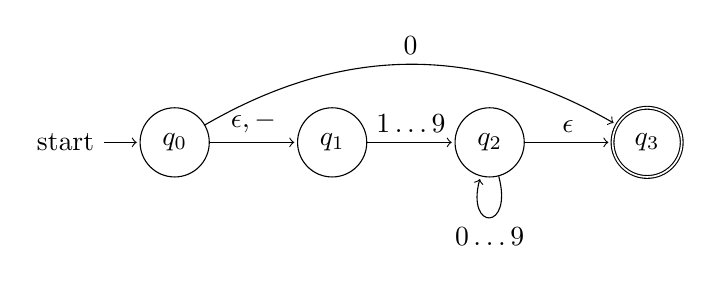
\begin{tikzpicture}[shorten >=1pt,node distance=2cm,on grid,auto]
    \node[state,initial] (q0) {$q_0$};
    \node[state] (q1) [right = of q0]{$q_1$};
    \node[state] (q2) [right = of q1]{$q_2$};
    \node[state,accepting] (q3) [right = of q2]{$q_3$};
    \path[->]
    (q0)
    edge [] node [] {$\epsilon,-$} (q1)
    edge [bend left] node [] {$0$} (q3)
    (q1)
    edge [] node [] {$1 \dots 9$} (q2)
    (q2)
    edge [loop below] node [] {$0 \dots 9$} ()
    edge [] node [] {$\epsilon$} (q3)
    ;
  \end{tikzpicture}
\end{center}

\begin{center}
  \begin{tabular}{c|cccc}
    $\delta$ & $\epsilon$  & $-$         & $0$         & $1 \dots 9$ \\ \hline
    $q_0$    & $q_1$       & $q_1$       & $q_3$       & $\emptyset$ \\
    $q_1$    & $\emptyset$ & $\emptyset$ & $\emptyset$ & $q_2$       \\
    $q_2$    & $q_3$       & $\emptyset$ & $q_2$       & $q_2$       \\
    $q_3$    & $\emptyset$ & $\emptyset$ & $\emptyset$ & $\emptyset$
  \end{tabular}
\end{center}

\begin{mydef}
  A subset $P \subset Q$ is $\epsilon$-close if all $\epsilon$-transitions from
  $P$ leads to $P$, that is for all $q \in P$, $\delta(q,\epsilon) \subset P$.
\end{mydef}

\begin{mydef}
  The $\epsilon$-closure $\overline P$ of $P$ is the minimal
  $\epsilon$-close subset containing $P$, the construction of $\overline{P}$ is
  done by induction :
  
  \textbf{Base case : } State $q$ is in $ECLOSE(q)$.
  
  \textbf{Induction : } If state $p$ is in $ECLOSE(q)$, and there is a
  transition from state $p$ to state $r$ labeled $\epsilon$, then $r$ is in $ECLOSE(q)$.
\end{mydef}

\begin{mydef}
  The extended transition function for an $\epsilon$-NFA $\widehat{\delta} : Q
  \times \Sigma^* \mapsto 2^Q$ is defined recursively as follows :
  $\widehat{\delta}(q,\epsilon) := \{q\}$ and if $\omega \in \Sigma^*$ and
  $|\omega| = n$, then $\omega = \omega_0a$ for $|\omega_0| = n-1$, $a \in
  \Sigma$, $\widehat{\delta}(q,\omega) =
  \overline{\delta(\widehat{\delta}(q,\omega_0),Q)}$, by definition $\delta(P,a)
  := \bigcup_{a \in P} \delta(q,a)$, $P \subset Q$.
\end{mydef}

\paragraph{Example : }

\begin{center}
  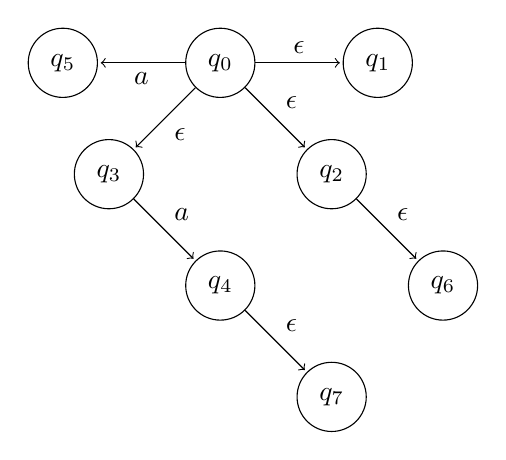
\begin{tikzpicture}[shorten >=1pt,node distance=2cm,on grid,auto]
    \node[state] (q0) {$q_0$};
    \node[state] (q1) [right = of q0]{$q_1$};
    \node[state] (q2) [below right = of q0]{$q_2$};
    \node[state] (q3) [below left = of q0]{$q_3$};
    \node[state] (q4) [below right = of q3]{$q_4$};
    \node[state] (q5) [left = of q0]{$q_5$};
    \node[state] (q6) [below right = of q2]{$q_6$};
    \node[state] (q7) [below right = of q4]{$q_7$};
    \path[->]
    (q0)
    edge [] node [] {$a$} (q5)
    edge [] node [] {$\epsilon$} (q1)
    edge [] node [] {$\epsilon$} (q2)
    edge [] node [] {$\epsilon$} (q3)
    (q1)
    (q2)
    edge [] node [] {$\epsilon$} (q6)
    (q3)
    edge [] node [] {$a$} (q4)
    (q4)
    edge [] node [] {$\epsilon$} (q7)
    ;
  \end{tikzpicture}
\end{center}

\begin{gather*}
  \widehat{\delta}(q,\epsilon) = \{q_0,q_1,q_2,q_3,q_6\} \\
  \widehat{\delta}(q,a) = \{q_5,q_4,q_7\} \\
\end{gather*}

\begin{mydef}
  The language accepted by an $\epsilon$-NFA $A$ is $L(A) = \{\omega \in
  \Sigma^* | \widehat{\delta}(q_0,\omega) \cap F \neq \emptyset\}$
\end{mydef}

\begin{thm}
  If $L$ is a language accepted by an $\epsilon$-NFA $A$, then there exists a
  DFA $D$ which accepts $L$.
\end{thm}

\begin{proof}
  \begin{align*}
    & A = (Q,\Sigma,\delta,q_0,F) \\
    & D = (2^Q,\Sigma,\delta',q_0',F') \\
    & q_0' = \{q_0\} \\
    & F' = \{P \subset Q | P \cap F \neq \emptyset\} \\
    & \delta'(P,a) = \overline{\delta(P,a)}
  \end{align*}

  Claim : $\widehat{\delta'}(q_0',\omega) = \widehat{\delta}(q_0,\omega)$
  \begin{align*}
    \omega \in L(A) &\iff \widehat{\delta}(q_0,\omega) \cap F \neq \emptyset \\
                    &\iff \widehat{\delta'}(q_0',\omega) \cap F \neq \emptyset \\
                    &\iff \widehat{\delta}(q_0,\omega) \cap F' \neq \emptyset \\
                    &\iff \omega \in L(D)
  \end{align*}
  Then $L(A) = L(D)$.

  Induction on the length :

  \paragraph{Base case : } $|\omega| = 0$, then $\omega = \epsilon$
  $\widehat{\delta'}(q_0',\epsilon) = q_0' = \{q_0\}$.
  
  \paragraph{Inductive step : } $|\omega| = n$, then $\omega = \omega_0 a$,
  $|\omega_0| = n-1$, $a \in \Sigma$

  \begin{align*}
    \widehat{\delta'}(q_0'\omega) &= \delta'(\widehat{\delta'}(q_0',\omega_0),a) \\
                                  &= \delta'(\widehat{\delta}(q_0,\omega_0),a) \\
                                  &= \delta(\widehat{\delta}(q_0,\omega_0),a) \\
                                  &= \widehat{\delta}(q_0,\omega)
  \end{align*}
\end{proof}

We transform

\begin{center}
  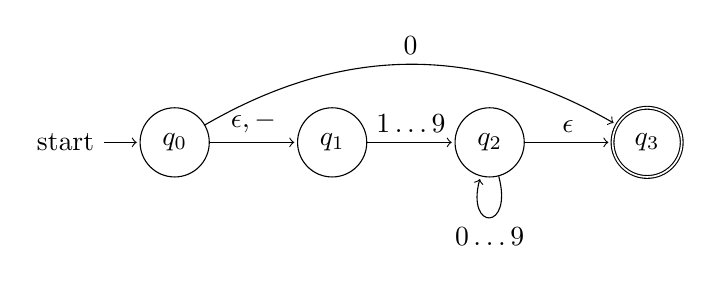
\begin{tikzpicture}[shorten >=1pt,node distance=2cm,on grid,auto]
    \node[state,initial] (q0) {$q_0$};
    \node[state] (q1) [right = of q0]{$q_1$};
    \node[state] (q2) [right = of q1]{$q_2$};
    \node[state,accepting] (q3) [right = of q2]{$q_3$};
    \path[->]
    (q0)
    edge [] node [] {$\epsilon,-$} (q1)
    edge [bend left] node [] {$0$} (q3)
    (q1)
    edge [] node [] {$1 \dots 9$} (q2)
    (q2)
    edge [loop below] node [] {$0 \dots 9$} ()
    edge [] node [] {$\epsilon$} (q3)
    ;
  \end{tikzpicture}
\end{center}

\[
  q_0' = \{q_0\} = \{q_0,q_1\}
\]

\begin{center}
  \begin{tabular}{c|ccc}
    $\delta$      & $-$         & $0$           & $1 \dots 9$   \\ \hline
    $\{q_0,q_1\}$ & $\{q_1\}$   & $\{q_3\}$     & $\{q_2,q_3\}$ \\
    $\{q_1\}$     & $\emptyset$ & $\emptyset$   & $\{q_2,q_3\}$ \\
    $\{q_3\}$     & $\emptyset$ & $\emptyset$   & $\emptyset$   \\
    $\{q_2,q_3\}$ & $\emptyset$ & $\{q_2,q_3\}$ & $\{q_2,q_3\}$ \\
    $\emptyset$   & $\emptyset$ & $\emptyset$   & $\emptyset$  
  \end{tabular}
\end{center}

\section{Regular expressions and regular languages}

\begin{mydef}
  Regular expressions (RE) denote languages
  \begin{enumerate}
  \item $\emptyset$ is a RE generating the empty language $\emptyset$ (two
    state, no transition, the initial state is not accepting).
  \item $\epsilon$ is a RE generating $\{\epsilon\}$ (one state, initial and final).
  \item $a \in \Sigma$ is a RE generating $\{a\}$.
  \item if $r$ and $s$ are RE generating $R$ and $S$, then $r + s$ is a RE
    generating the language $R \cup S$.
  \item if $r$ and $s$ are RE generating $R$ and $S$, then $r \cdot s$ is a RE
    generating $RS = \{uv | u\in R\ \wedge\ v \in S\}$
  \item if $r$ is a RE generating $R$, then $r^*$ is a RE generating $R^* =
    \bigcup_{i=0}^\infty R^i$, $R^i = \underbrace{RRR\dots R}_{i\text{ times}}$,
    $R^0 = \epsilon$. Its called the Kleene closure of $R$.
  \item Priority operation : $* > \cdot > +$
  \end{enumerate}
\end{mydef}

\begin{thm}
  A language $L$ is accepted by some DFA if and only if it is denoted by a
  regular expression.
\end{thm}

\begin{lemma}
  For a regular expression $r$, there is an $\epsilon$-NFA $M$ such that it
  accepts $R = L(r)$ and it has only one final state without any transition from it.
\end{lemma}

\begin{proof}
  Induction on the number of operation in $r$ :
  
  \textbf{Base : }
  \begin{enumerate}
  \item $r = \emptyset$ : two state and no transition, the initial state is not final.
  \item $r = \epsilon$ : one state which is final.
  \item $r = a \in Sigma$ : two state and one transition labeled $a$, the
    initial state is not final but the other is.
  \end{enumerate}

  \textbf{Inductive step : }
  \begin{enumerate}
  \item $r = r_1 + r_2$ : $R = R_1 \cup R_2$ $\to$ if $\omega$ is accepted by $M$ $\iff$ $\omega \in R_1
    \vee \omega \in R_2$.
    
    \begin{center}
      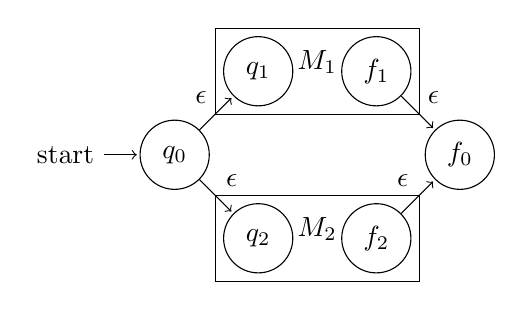
\begin{tikzpicture}[shorten >=1pt,node distance=1.5cm,on grid,auto]
        \node[state,initial] (q0) {$q_0$};
        \node[state] (q1) [above right = of q0]{$q_1$};
        \node[state] (q2) [below right = of q0]{$q_2$};
        \node[state] (f1) [right = of q1]{$f_1$};
        \node[state] (f2) [right = of q2]{$f_2$};
        \node[state] (f0) [below right = of f1]{$f_0$};
        \node[draw=black, fit= (q1) (f1), inner sep=0.1cm] {$M_1$};
        \node[draw=black, fit= (q2) (f2), inner sep=0.1cm] {$M_2$};
        \path[->]
        (q0)
        edge [] node [] {$\epsilon$} (q1)
        edge [] node [] {$\epsilon$} (q2)
        (q1)
        (q2)
        (f0)
        (f1)
        edge [] node [] {$\epsilon$} (f0)
        (f2)
        edge [] node [] {$\epsilon$} (f0)
        ;
      \end{tikzpicture}
    \end{center}

  \item $r = r_1 \cdot r_2$ : $R = R_1R_2$ $\to$ if $\omega \in R_1R_2$ $\iff$
    $\omega = \omega_1\omega_2$ $\iff$ $\omega$ accepted by $M$.

    \begin{center}
      \begin{tikzpicture}[shorten >=1pt,node distance=2cm,on grid,auto]
        \node[state,initial] (q1) {$q_1$};
        \node[state] (f1) [right = of q1]{$f_1$};
        \node[state] (q2) [right = of f1]{$q_2$};
        \node[state,accepting] (f2) [right = of q2]{$f_2$};
        \node[draw=black, fit= (q1) (f1), inner sep=0.1cm] {$M_1$};
        \node[draw=black, fit= (q2) (f2), inner sep=0.1cm] {$M_2$};
        \path[->]
        (q0)
        (q1)
        (q2)
        (f0)
        (f1)
        edge [] node [] {$\epsilon$} (q2)
        (f2)
        ;
      \end{tikzpicture}
    \end{center}
    
  \item $r = r_1*$ : $R = R_1^* = \bigcup_{i=0}^\infty R^i$, if $\omega \in
    R_i^* \iff \omega = \omega_1 \dots \omega_k \iff \omega$ accepted by $M$.
    
    \begin{center}
      \begin{tikzpicture}[shorten >=1pt,node distance=2cm,on grid,auto]
        \node[state,initial] (q0) {$q_0$};
        \node[state] (q1) [right = of q0]{$q_1$};
        \node[state,accepting] (f1) [right = of q1]{$f_1$};
        \node[state] (f0) [right = of f1]{$f_0$};
        \node[draw=black, fit= (q1) (f1), inner sep=0.1cm] {$M_1$};
        \path[->]
        (q0)
        edge [bend right] node [] {$\epsilon$} (f0)
        edge [] node [] {$\epsilon$} (q1)
        (q1)
        (q2)
        (f0)
        (f1)
        edge [bend right] node [above] {$\epsilon$} (q1)
        edge [] node [] {$\epsilon$} (f0)
        (f2)
        ;
      \end{tikzpicture}
    \end{center}
    
  \end{enumerate}
  
\end{proof}

\begin{lemma}
  For a DFA $M$, there is a regular expressions $r$ describing the language $R =
  L(M)$.
\end{lemma}

\begin{proof}
  Assume that $M's$ states are $\{1,2,\dots,n\}$ for some integer $n$. No
  matter what the states of $A$ actually are, there will be $n$ of them for some finite
  $n$ , and by renaming the states, we can refer to the states in this manner, as if
  they were the first $n$ positive integers.

  Denote by $R_{ij}^{(k)}$ the name of a regular expression whose language is the
  set of strings $\omega$ such that $\omega$ is the label of a path from state $i$
  to state $j$ in $A$, and that path has no intermediate node whose number is
  greater than $k$. Note that the beginning and end points of the path are not
  ``intermediate'', so there is no constraint that $i$ and/or $j$ be less than or
  equal to $k$.

  To construct the expressions $R_{ij}^{(k)}$, we use the following inductive
  definition, starting at $k=0$ and finally reaching $k=n$. When $k = n$, there is
  no restriction at all on the paths represented, since there are no states
  greater than $n$.

  \textbf{Base : } $k = 0$
  \begin{itemize}
  \item $i \neq j$ and $R_{ij}^0 = \emptyset \implies r_{ij}^0 = \emptyset$.
  \item $i \neq j$ and $R_{ij}^0 = \{a_1,\dots,a_m\} \implies r_{ij}^0 = a_1 + a_2
    + \dots + a_m$.
  \item $i = j$ and  $R_{ij}^0 = \{\epsilon\} \implies r_{ij}^0 = \epsilon$
  \item $i = j$ and $R_{ij}^0 = \{a_1,\dots,a_m\} \implies r_{ij}^0 = a_1 + a_2 +
    \dots + a_m + \epsilon$
  \end{itemize}

  \textbf{Inductive step : } Suppose there is a path from state $i$ to state $j$
  that goes through no state higher than $k$. There are two possible cases to
  consider :

  \begin{enumerate}
  \item The path does no go through state $k$ at all. In this case, the label of
    the path is in the language if $R_{ij}(k-1)$.
  \item The path goes through state $k$ at least once, then we can break the path
    into several pieces. The first piece goes from state $i$ to $k$ and the last
    piece goes from $k$ to $j$ without passing through $k$, and all the pieces in
    the middle go from $k$ to itself, without passing through $k$. The set of
    labels for all paths of this type is represented by the regular expression
    $R_{ik}^{(k-1)}(R_{kk}^{(k-1)})^* R_{kj}^{(k-1)}$.
  \end{enumerate}

  When we combine the expressions for the paths of the two types above, we have
  the expression

  \[
    R_{ik}^{(k)} = R_{ij}^{(k-1)} + R_{ik}^{(k-1)} (R_{kk}^{(k-1)})^* R_{kj}^{(k-1)}
  \]

  The regular expression for the language of the automaton is then the sum (union)
  of all expressions $R_{1j}^{(n)}$ such that $j$ is an accepting state.
\end{proof}

\begin{thm}
  Assume that $L$ is a regular language, then $\Sigma^* \setminus L$ is a
  regular language.
\end{thm}

\begin{proof}
  \begin{align*}
    & \exists M : DFA, L = L(M), M = (Q,\Sigma,\delta,q_0,F) \\
    & M' = (Q,\Sigma,\delta,q_0, Q \setminus F) \text{ accepts } \Sigma^* \setminus L \\
    & \omega \in \Sigma^* \setminus L \iff \omega \not \in L \iff \widehat{\delta}(q_0,\omega) \not \in F \iff \widehat{\delta}(q_0,\omega) \in Q \setminus F
  \end{align*}
\end{proof}

\begin{cor}
  If $L_1$ and $L_2$ are regular languages, then $L_1 \cap L_2$ is a regular
  language and $L_1 \setminus L_2$ is a regular language.
\end{cor}

\begin{proof}($L_1 \cap L_2$ is a regular language)
  We know that $L_1 \cup L_2$ is a regular language. Therefore, we have
  \[
    L_1 \cap L_2 = \overline{\overline{L_1} \cup \overline{L_2}}, \text{where }
    \overline{L} = \Sigma^* \setminus L
  \]
\end{proof}

\begin{proof}($L_1 \setminus L_2$ is a regular language)
  \[
    L_1 \setminus L_2 = L_1 \cap \overline{L_2}
  \]
\end{proof}

\section{The pumping lemma and homomorphisms}

Can we decide algorithmically whether two given automata or two given RE define
the same language ? It suffices to give a positive answer to one of those
questions, because we have algorithms for automaton $\leftrightarrow$ RE.

\begin{thm}
  There is an algorithm that decide whether two given automata are equivalent.
\end{thm}

\begin{proof}
  Let $M_1$ and $M_2$ be two automata, and $L_1= L(M_1)$, $L_2 = L(M_2)$.
  Consider the symmetric difference : $L_1 \triangle L_2 = (L_1 \setminus L_2)
  \cup (L_2 \setminus L_1)$, $L_1,L_2$ regular $\implies L_1 \triangle L_2$
  regular.

  Let $M$ be a finite automaton that accepts the language $L_1 \triangle L_2$,
  it suffices to decide if $L(M)$ is empty or not, but $L(M) = \emptyset \iff $
  there is no path from $q_0$ to $F$
\end{proof}

\begin{thm}[The pumping lemma for regular languages]
  Let $L$ be a regular language, then there is a positive integer $n$ such that
  any word $z \in L$ of length $|z| \geq n$ can be written as $z = uvw$ in such
  a way that $|uv| \leq n$, $|v| \geq 1$ and $\forall k \geq 0 : uv^kw \in L$.
\end{thm}

\begin{proof}
  Take a DFA that accepts $L$, let $n$ be the number of its states. Take for
  $i,j$ tje first pair where the coincidence occurs. Then $j \leq n$.
\end{proof}

\paragraph{Example : } $\Sigma = \{0\}, L = \{0^P\ |\ p\ prime\}$,
then $L$ is non-regular.

There are large gaps between the primes : $n!+ 2, n! + 3, \dots, n! + n$ are all
composite (non-prime). Take $k$ such that $p_{k+1} > p_k + n$, $0^{p_k} \in L $
(assume $L = L(M)$ and $|Q|=n$), $0^{p_k} = \underbrace{uvw}_{v=0^l,l \leq n},\
uv^2w = o^{p_k + p},\ p_k + p \leq p_k + n < p_k + 1 \implies uv^2w \not \in L$.

\begin{thm}
  A language accepted by a DFA with $n$ states is
  \begin{enumerate}
  \item non-empty if an only if it contains a word of length $< n$.
  \item infinite if and only if it contains a word of length $l$, where $n \leq
    l \leq 2n$.
  \end{enumerate}
\end{thm}

\begin{proof}
  \white{AD}
  \begin{enumerate}
  \item A shortest word in $L$ has length $< n$, otherwise it revisits some
    state and can be shortened.
  \item \begin{itemize}
    \item Assume $z \in L$ and $|z| \geq n$, then $z = uvw \implies uv^kw \in L
      \implies L\ infinite$.
    \item Assume $L$ is infinite, then $\exists z \in L$ such that $|z| \geq n$.
      \begin{itemize}
      \item If $|z| < 2n$, then done.
      \item If $|z| \geq 2n$, tjen by the pumping lemma
        \[
          z = uvw,\ 1 \geq |v| \geq n,\ uw \in L
        \]
        We have $|uw| = |z| - |v| \geq |z| - n \geq n$
      \end{itemize}
    \end{itemize}
  \end{enumerate}
\end{proof}

\begin{mydef}
  Let $\Sigma,\Delta$ be finite alphabets, a homomorphisms is a map $h :
  \Sigma^* \mapsto \Delta^*$ such that $h(xy) = h(x) h(y) \forall x,y \in \Sigma^*$.
\end{mydef}

\begin{lemma}
  A homomorphisms is uniquely determined by the images of letters of $\Sigma$.
  That is, any $h : \Sigma \mapsto \Delta^*$ extends to a unique homomorphisms.
\end{lemma}

\begin{proof}
  \white{Hello}
  \begin{itemize}
  \item Uniqueness : assume $h(a)$ is given $\forall a \in \Sigma$, then for
    $\omega = a_1a_2\dots a_n$, we have no other choice but $h(\omega) =
    h(a_1)h(a_2)\dots h(a_n)$, $h(\epsilon) = \epsilon$ and $h(x) = h(x\epsilon)
    = h(x)h(\epsilon) \implies h(\epsilon) = \epsilon$.
  \item Existence : $h(\omega) = h(a_1)h(a_2)\dots h(a_n)$ defines a homomorphisms.
  \end{itemize}
\end{proof}

\paragraph{Example : } $\Sigma = \Delta = \{0\}$, $L = \Sigma^*$
\[
  h(0) = 00 \implies h(L) = \{\text{all words of even length}\}
\]

\paragraph{Example : } $\Sigma = \Delta = \{0,1\}$, $L = \Sigma^*$

\begin{gather*}
  h(0) = 0 \\
  h(1) = 10 \\
  h(L) = ? \\
  L = (0+1)^* \\
  h(L) = (0+10)^*
\end{gather*}

\begin{thm}
  A homomorphic image of a regular language is regular
\end{thm}

\begin{proof}
  Let $L$ be a regular language and $r$ a regular expression generating $L$.
  Replace in $r$ every letter by its image under $h$. The result is a regular
  expression. This expression represents the language $h(L)$. Proof by induction
  on the complexity if $r$.
\end{proof}

\paragraph{Note : } a homomorphisms image of a non-regular language might be
regular.

\begin{mydef}
  Given a homomorphisms $h: \Sigma^* \mapsto \Delta^*$ and $L \cup \Delta^*$,
  the inverse homomorphic image of $L$ is :
  \[
    h^{-1}(L) = \{\omega \in \Sigma^* | h(\omega) \in L\}
  \]
\end{mydef}

\paragraph{Example : } $\Sigma = \{a,b\}$ $\Delta = \{0,1\}$
\begin{gather*}
  L = (00 + 1)^* \\
  h(a) = 01 \\
  h(b) = 10 \\
  h^{-1}(1001) = \{ba\} \\
  h^{-1}(L) = \text{all words in $a,b$ such that after the 0's come in pairs}
\end{gather*}

\begin{itemize}
\item cannot begin with $a$
\item it has to begin with $b$
\end{itemize}
\[
  \implies (ba)^* = h^{-1}(L)
\]

\begin{thm}
  Regular language are closed under inverse homomorphisms.
\end{thm}

\begin{proof}
  Let $M = (Q,\Delta,\delta,q_0,F)$ be a DFA for $L$, then construct $M' =
  (Q,\Sigma,\delta',q_0,F)$ such that $L(M') = h^{-1}(L)$.
  \[
    \delta'(q_0,a) = \widehat{\delta}(q_0,h(a)) \implies \forall w \in \Sigma^*
    : \widehat{\delta'}(q_0,\omega) = \widehat{\delta}(q_0,h(w))
  \]
  \[
    \omega \in L(M') \iff \widehat{\delta}(q_0,h(\omega)) \in F \iff h(\omega)
    \in L(M)
  \]
\end{proof}

\section{The Myhill-Nerode theorem}

\begin{mydef}
  Let $L \subset \Sigma^*$ be any language. We say that $u,v \in \Sigma^*$ are
  $L-$equivalent ($u \sim_L v$) if $\forall x \in \Sigma^* : (ux,vx \in L) \vee
  (ux,vx \not \in L)$.

  \textbf{Note : } or $u \not \sim_L v \iff \exists \text{ distinguisting
    extension } x \in \Sigma^* \text{ ,that is exactly one of $ux$, $vx$ is in $L$}$.
\end{mydef}

\begin{lemma}
  $\sim_L$ is an equivalence relation :
  \begin{itemize}
  \item reflexive : $u \sim_L u$.
  \item symetric : $u \sim_L v \implies v \sim_L u$.
  \item transitive : $u \sim_L v \wedge v \sim_L w \implies u \sim_L w$.
  \end{itemize}
\end{lemma}

\begin{proof}(transitivity)
  
  Assume $u \not \sim_L w$.

  Take $x$ such that, without lost of generality, $ux \in L$ and $wx \in L$, now
  \begin{itemize}
  \item $vx \in L \implies v \not \sim_L w$
  \item $vx \not \in L \implies u \not \sim_L v$
  \end{itemize}
\end{proof}

\begin{cor}
  $\Sigma^*$ splits into equivalence classes :
  
  \[
    \Sigma^* = \bigcup_i S_i
  \]

  where $u \sim_L v \iff \exists i \ s.t.\ u,v \in S_i$
\end{cor}

\paragraph{Example : } $L \ subset \{0,1\}^* \quad L = \{w |
\underbrace{l_0(w)}_{\text{number of $0$ in $w$}} \text{ is not divisible by }
3\}$

Then

\[
  u \sim_L v \iff l_0(u) \equiv l_0(v) \mod 3 \\
\]
\begin{align*}
  l_0(u) &= 2 l_0(ux) &= l_0(u) + l_0(x) &= l_0(x) + 2 \\
  l_0(v) &= 5 l_0(vx) &= l_0(v) + l_0(x) &= l_0(x) + 5 \\
\end{align*}
\begin{align*}
  \Sigma^* &= S_0 \cup S_1 \cup S_2 \\
  S_i &= \{w | l_0(w) \equiv i \mod 3\} \\
  L &= S_1 \cup S_2
\end{align*}

\begin{lemma}
  \[
    u \sim_L v \implies u,v \in L \vee u,v \not \in L
  \]

  \textbf{The converse is not true.}
\end{lemma}

\begin{proof}
  Put $x = \epsilon$ in the definition.
\end{proof}

\begin{cor}
  \[
    \forall S_i : \text{either} S_i \subset L \text{ or } S_i \cap L = \emptyset
  \]
\end{cor}

\paragraph{Example : } $L = \{w\ |\ l_0(w) = l_1(w)\}$
\[
  u \sim_L v \iff l_0(u) - l_1(u) = l_0(v) - l_1(v)
\]
follows from $l_0(ux) = l_0(u) + l_0(x) \dots$

\begin{lemma}
  If $u \sim_L v$, then $\forall a : \Sigma$, we have $ua \sim_L va$ ($\sim_L$
  is right invariant).
\end{lemma}

\begin{proof}
  Assume $ua \sim_L va$, take a distinguishing extension $x$, without lost of
  generality, we have $vax \in L, vax \not \in L$. Then $ax$ is a distinguishing
  extension for $u,v$.
\end{proof}

\paragraph{Remark : } the converse is false : $ua \sim_L va \not \implies u
\sim_L v$
\paragraph{Example : } $L = (0 + 1)^* 0$, $10 \sim_L 00$, but $1 \not \sim_L 0$.

\[
  x = \epsilon \implies u \not \in L \wedge v \in L
\]

\begin{thm}[Myhill-Nerode]
  A language $L$ is regular if and only if the number of $L$-equivalence classes
  is finite.
\end{thm}

\begin{proof}
  Assume $\Sigma^* = S_1 \cup S_2 \cup \dots \cup S_n, \epsilon \in S_1$. We
  will construct a DFA with n states accepting $L$. $Q = \{q_1,\dots,q_n\}$
  where $q_1$ is the initial state and $q_i$ a final state such that $q_i(final)
  \iff S_i \subset L$.

  To find $\delta(q_i,a)$, take any $v \in S_i$ and look where $va$ is :

  \[
    \delta(q_i,a) = q_j, \text{ where } va \in S_j
  \]

  $\widehat{\delta}(q_1,w) = q_i$ where $w \in S_i$ (choosing $\epsilon \in
  S_1$) $w = a_1 \dots a_n$, $w \in L(M) \iff q_i \text{ final} \iff S_i \subset
  L \iff w \in L$.

  Assume $L$ is regular and take a DFA $M$ accepting $L$. Put $T_i = \{w \in
  \Sigma^* | \widehat{\delta}(q_1,w) = q_i\}$. These are equivalence classes
  with respect to $u \sim_M v \iff \widehat{\delta}(q_1,u) =
  \widehat{\delta}(q_1,v)$.

  \begin{claim}
    $u \sim_M v \implies u \sim_L v$
  \end{claim}

  Have $\widehat{\delta}(q_1,u) = \widehat{\delta}(q_1,v)$, then

  \begin{align*}
    \widehat{\delta}(q_1,ux) &= \widehat{\delta}(\widehat{\delta}(q_1,u),x) \\
                             &= \widehat{\delta}(\widehat{\delta}(q_1,v),x) \\
                             &= \widehat{\delta}(q_1,vx) \\
                             && \implies \text{ either both $ux,vx \in L$ or both $ux,vx \not \in L$} \\
  \end{align*}

  This holds $\forall x \implies u \sim_L v$. It follows that every $T_i$ is
  contained in some $S_j$ $\implies$ the number of $L$-equivalence classes is
  finite and $\leq m$.
\end{proof}

\begin{thm}
  The minimum number of states in a DFA accepting $L$ is equal to $ind(L)$
  (index of $L$, its number of equivalence classes). The minimal automaton is
  unique (up to renaming the states).
\end{thm}

\begin{proof}
  From the end of the last proof, $|Q| \geq ind(L)$. For any DFA accepting $L$ :
  \begin{itemize}
  \item From the $1^{\text{st}}$ half of the Myhill-Nerode theorem, there is a
    DFA $M$ with $ind(L)$ states.
  \item For any DFA with $|Q| = ind(L)$, every $T_i$ is equal to some $S_j$.
  \item One can see that $\delta$ for $M$ coincides with $\delta$ defined for $S_1,\dots,S_n$
  \end{itemize}
\end{proof}

\paragraph{Algorithm to minimize DFA}

\begin{center}
  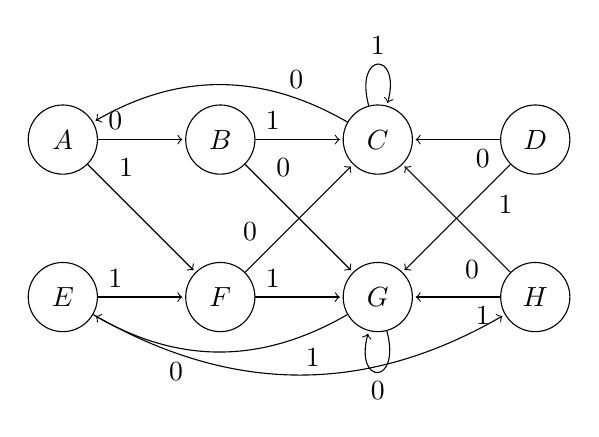
\begin{tikzpicture}[shorten >=1pt,node distance=2cm,on grid,auto]
    \node[state] (A) {$A$};
    \node[state] (B) [right = of A]{$B$};
    \node[state] (C) [right = of B]{$C$};
    \node[state] (D) [right = of C]{$D$};
    \node[state] (E) [below = of A]{$E$};
    \node[state] (F) [right = of E]{$F$};
    \node[state] (G) [right = of F]{$G$};
    \node[state] (H) [right = of G]{$H$};
    \path[->]
    (A)
    edge [] node [pos = 0.2] {$0$} (B)
    edge [] node [pos = 0.2] {$1$} (F)
    (B)
    edge [] node [pos = 0.2] {$0$} (G)
    edge [] node [pos = 0.2] {$1$} (C)
    (C)
    edge [bend right] node [above,pos = 0.2] {$0$} (A)
    edge [loop above] node [] {$1$} ()
    (D)
    edge [] node [pos = 0.2] {$0$} (C)
    edge [] node [pos = 0.2] {$1$} (G)
    (E)
    edge [bend right] node [below, pos = 0.2] {$0$} (H)
    edge [] node [pos = 0.2] {$1$} (F)
    (F)
    edge [] node [pos = 0.2] {$0$} (C)
    edge [] node [pos = 0.2] {$1$} (G)
    (G)
    edge [loop below] node [] {$0$} ()
    edge [bend left] node [pos = 0.2] {$1$} (E)
    (H)
    edge [] node [pos = 0.2] {$0$} (C)
    edge [] node [pos = 0.2] {$1$} (G)
    ;
  \end{tikzpicture}
\end{center}

\begin{center}
  \begin{tabular}{|c|c|cccccc}
    \cline{1-2}
    B & {\color{green}$\times$} &  &  &  &  &  &  \\ \cline{1-3}
    C & $\times$ & \multicolumn{1}{c|}{$\times$} &  &  &  &  &  \\ \cline{1-4}
    D & {\color{green}$\times$} & \multicolumn{1}{c|}{{\color{green}$\times$}} & \multicolumn{1}{c|}{$\times$} &  &  &  &  \\ \cline{1-5}
    E &  & \multicolumn{1}{c|}{{\color{green}$\times$}} & \multicolumn{1}{c|}{$\times$} & \multicolumn{1}{c|}{{\color{green}$\times$}} &  &  &  \\ \cline{1-6}
    F & {\color{green}$\times$} & \multicolumn{1}{c|}{{\color{green}$\times$}} & \multicolumn{1}{c|}{$\times$} & \multicolumn{1}{c|}{} & \multicolumn{1}{c|}{{\color{green}$\times$}} &  &  \\ \cline{1-7}
    G & {\color{red}$\times$} & \multicolumn{1}{c|}{{\color{green}$\times$}} & \multicolumn{1}{c|}{$\times$} & \multicolumn{1}{c|}{{\color{green}$\times$}} & \multicolumn{1}{c|}{{\color{red}$\times$}} & \multicolumn{1}{c|}{{\color{green}$\times$}} &  \\ \hline
    H & {\color{green}$\times$} & \multicolumn{1}{c|}{} & \multicolumn{1}{c|}{$\times$} & \multicolumn{1}{c|}{{\color{green}$\times$}} & \multicolumn{1}{c|}{{\color{green}$\times$}} & \multicolumn{1}{c|}{{\color{green}$\times$}} & \multicolumn{1}{c|}{{\color{green}$\times$}} \\ \hline
      & A & \multicolumn{1}{c|}{B} & \multicolumn{1}{c|}{C} & \multicolumn{1}{c|}{D} & \multicolumn{1}{c|}{E} & \multicolumn{1}{c|}{F} & \multicolumn{1}{c|}{G} \\ \hline
  \end{tabular}
\end{center}

\begin{proof}[Algorithm]
  \white{induction}
  
  \textbf{Base : } if $p \in F$ and $q \not \in F$, then mark $(p,q)$.
  
  \textbf{Inductive step : } $\forall (p,q)\ s.t.\ (p,q)\ \text{not marked}$ and
  $\forall a$ if $(\delta(p,a),\delta(q,a))$, then mark $(p,q)$. Stop when no
  more pairs are marked.
\end{proof}

\section{Context-free grammars}

\begin{mydef}
  A context-free grammar (CFG, or just grammar) is $G = (V,T,P,S)$ where
  \begin{itemize}
  \item $V$ is a finite set of variables.
  \item $T$ is a finite set of terminals.
  \item $P$ is a finite set of productions of the form $A \to \alpha$, where $A
    \in V$, $\alpha \in (V \cup T)^*$.
  \item $S \in V$ a special variable called start symbol.
  \end{itemize}
\end{mydef}

\paragraph{Convention on notation : }
\begin{itemize}
\item Capitals $A,B,C,D,\dots$ are variables.
\item lowercase $a,b,c,d,\dots$ and digits are terminals.
\item $\alpha,\beta,\gamma \in (V \cup T)^*$ are strings of variables and terminals.
\item $u,v,w,x,y,z \in T^*$ are strings of terminals.
\end{itemize}

\begin{mydef}
  If $A \to \beta$ is a production in $G$, then we write $\alpha A \gamma
  \Rightarrow_{G} \alpha \beta \gamma$ and say : ``$\alpha A \gamma$ directly
  derives $\alpha \beta \gamma$''.

  If $\alpha_1,\dots,\alpha_n \in (V \cup T)^*$ such that
  \[
    \alpha_1 \Rightarrow_{G} \alpha_2, \alpha_2 \Rightarrow_{G} \alpha_3, \dots, \alpha_{n-1} \Rightarrow_{G} \alpha_n
  \]

  then $\alpha_1 \Rightarrow_G^* \alpha_n$, ``$\alpha_1$ derives $\alpha_n$''
  $\implies \Rightarrow^*$ if $G$ is understood.
\end{mydef}

\begin{mydef}
  The language generated by $G$ is the set of all strings of terminals that can
  be derived from the start symbol :
  \[
    L(G) = \{\omega \in T^* | S \Rightarrow_G^* \omega \}
  \]
\end{mydef}

\paragraph{Example : } $S \to (S \wedge S)\  |\  (S \vee S)\  |\  (\neg S)\  |\  p\  |\  q$
generates propositional formulas in $p$ and $q$.

\begin{mydef}
  Grammars $G$ and $G'$ are called equivalent if $L(G) =) L(G')$.
\end{mydef}

\begin{mydef}
  A symbol $X \in V \cup T$ is called useful if it is used in a derivation of
  some word in $L(G)$, if this is a derivation of the form :
  \[ 
    S \Rightarrow^* \alpha X \beta \Rightarrow^* \omega, \text{ where $\omega$
      is composed of words and terminals only}
  \]
  
  A symbol $X$ is called generating if $X \Rightarrow^* \omega$ for some
  $\omega$. Any $a \in T$ is generating.

  A symbol $X$ is called reachable if
  \[
    S \Rightarrow^* \alpha X \beta \text{ for some }  \alpha,\beta \in (V \cup T)^*
  \]

  Then, useful means that the symbol is reachable and generating, $\alpha X
  \beta \Rightarrow^* \omega \implies X \Rightarrow^* v, \text{where $v$ is a
    subword of $\omega$}$.
\end{mydef}

\begin{thm}
  Let $G$ be a CFG, then there is a CFG $G''$ such that $L(G'') = L(G)$ and
  $G''$ has no useless symbols.

  \textbf{Construction : } Let $G = (V,T,P,S)$
  \begin{enumerate}
  \item Construct $G' = (V',T',P',S)$
    \begin{itemize}
    \item elimination from $V$ and $T$ of all non-generating symbols.
    \item elimination from $P$ of all production that contains non-generating symbols.
    \end{itemize}
  \item Construct $G''$ by elimination from $G'$ of all symbols non-reachable in
    $G'$ and all production with these symbols.
  \end{enumerate}
\end{thm}

\begin{proof}
  Suppose $X$ is a symbol that remains ($X \in V_1 \cup T_1$). We know that $X
  \Rightarrow_G^* \omega$ for some $\omega$ in $T^*$. Moreover, every symbol
  used in the derivation of $\omega$ from $X$ is also generating. Thus, $X
  \Rightarrow_{G''}^* \omega$
  
  Since $X$ was not eliminated in the second step, we also know that there are
  $\alpha$ and $\beta$ such that $S \Rightarrow_{G''}^* \alpha X \beta$.
  Further, every symbol used in this derivation is reachable, so $S
  \Rightarrow_{G'}^* \alpha X \beta$.

  We know that every symbol in $\alpha X \beta$ is reachable, and we also know
  that all these symbols are in $V_2 \cup T_2$, so each of them is generating in
  $G''$. The derivation of some terminal string, say $\alpha X \beta
  \Rightarrow_{G''}^* xwy$ , involves only symbols that are reachable from $S$,
  because they are reached by symbols in $\alpha X \beta$. Thus, this derivation
  is also a derivation of $G'$; that is,

  \[
    S \Rightarrow_{G'}^* \alpha X \beta \Rightarrow_{G'}^* xwy
  \]

  We conclude that $X$ is useful in $G'$. Since $X$ is an arbitrary symbol of
  $G'$, we conclude that $G'$ has no useless symbols.

  The last detail is that we must show $L(G_1) = L (G)$. As usual, to show two
  sets the same, we show each is contained in the other.

  \begin{itemize}
  \item $L(G_1) \subseteq L(G)$ : Since we have only eliminated symbols and
    productions from $G$ to get $G'$, it follows that $L(G_1) \subseteq L(G)$.
  \item $L(G_1) \supseteq L(G)$ : We must prove that if $\omega \in L(G)$, then
    $\omega \in L(G')$. If $\omega \in L(G)$, then $S \Rightarrow_{G}^* \omega$.
    Each symbol in this derivation is evidently both reachable and generating, so
    it is also a derivation of $G'$. That is, $S \Rightarrow_{G'}^* \omega$, and
    thus $\omega \in L(G_1)$.
  \end{itemize}
\end{proof}

\begin{thm}
  Let $G$ be a context free grammar, then $\exists G' : L(G') = L(G) \setminus
  \{\epsilon\}$ and $G'$ has no $\epsilon$-productions.
\end{thm}

\begin{proof}[Algorithm]
  \white{two setps}
  \begin{enumerate}
  \item Identify nullable variables, those $A$ for which $A \Rightarrow_G^*
    \epsilon$, by recursion :
    \begin{itemize}
    \item $A \to \epsilon \implies A \text{ is } nullable$.
    \item $A \to B_1,\dots,B_n \wedge B_1,\dots,B_n \text{ are } nullable
      \implies A \text{ is } nullable$.
    \end{itemize}
  \item Remove all $\epsilon$-productions and add new productions : Let $A \to
    X_1 \dots X_n$ be a production from $G$ with $n$ nullable variables among
    $X_1,\dots,X_n$. Add production of the form $A \to X_1 \dots X_n$, any
    subset of nullable variables is removed. There are $2^m$ productions.
  \end{enumerate}

  \textbf{Exception : } if all $X_i$ are nullable variable, then don't remove
  all of them at the same time.
\end{proof}

\paragraph{Example : } $S \to AB \quad A \to aAA\ |\ \epsilon \quad B \to bBB\
|\ \epsilon$, nullable : $S,A,B$ :
\[
  S \to AB\ |\ A\ |\ B \quad A \to aAA\ |\ aA\ |\ a \quad B \to bBB\ |\ bB\ |\ b
\]

\begin{thm}
  Let $G$ be a context free grammar, then $\exists G'$ such that $L(G') = L(G)$
  and $G'$ has no unit production, where an unit production is a production of
  the form $A \to B$.
\end{thm}

\begin{proof}[Algorithm]
  \white{two steps}
  \begin{enumerate}
  \item Identify unit pairs : $(A,B)$ such that $A \Rightarrow_G^* B$, note that
    $(A,A)$ is a unit pair.
  \item $\forall$ unit pair $(A,B)$ and $\forall$ non-unit pair $B \to \alpha$,
    form $A \to \alpha$. Let $P'$ be the set of all productions formed in this
    way, construct $G'=(V,T,P',S)$. $P'$ contains all non-unit production from $P$.
  \end{enumerate}
\end{proof}

\begin{thm}
  Let $G$ be a context free grammar that contains at least one non-empty word,
  then $\exists G' : L(G') = L(G) \setminus \{\epsilon\}$ and $G'$ has no
  useless symbols, no $\epsilon$-production and no unit-productions.
\end{thm}

\begin{proof}[Algorithm]
  \white{3 steps}
  \begin{enumerate}
  \item Eliminate $\epsilon$-productions.
  \item Eliminate unit-productions.
  \item Eliminate useless symbols.
  \end{enumerate}
\end{proof}

\begin{mydef}
  A grammar $G$ is in a Chomsky normal form is all its productions are of the
  form $A \to BC$ and $A \to a$.
\end{mydef}

\begin{thm}
  Any context free language without $\epsilon$ can be generated by a grammar in
  a Chomsky normal form.
\end{thm}

\begin{proof}
  By previous theorem, $\exists G' : L(G') = L(G)$ without
  $\epsilon$-productions and unit-productions. Any productions with one symbol
  at the right is $A \to a$, thus admissible.

  \begin{enumerate}
  \item Take any $A \to X_1 \dots X_n$, where $n \geq 2, X \in V \cup T$. Get ride of
    the terminals : if $X_i = a$, then introduce a new variable $C_a$ and $C_a \to
    a$. In $A \to X_1 \dots X_n$, replace $X_i$ by $C_a$.
  \item Now all productions are either $A \to a$ or $A \to B_1 \dots B_n, B_i
    \in V$, for all productions of the form $A \to B_1 \dots B_n$, introduce new
    variables $D_1,\dots,D_{n-2}$ and replace $A \to B_1 \dots B_n$ by $A \to
    B_1D_1, D_1 \to B_2D_2, \dots, D_{n-2} \to B_{n-1}B_{n}$.
  \end{enumerate}
\end{proof}

\section{Pushdown automata}

\begin{thm}
  Context-free languages are closed under union, concatenation and Kleene closure.
\end{thm}

\begin{proof}
  Take $L_1 = L(G_1)$ and $L_2 = L(G_2)$, $G_i = (V_i,T_i,P_i,S_i)$. We can
  assume that $V_1 \cap V_2 = \emptyset$ (otherwise rename variables, but don't
  rename terminals). New alphabet of terminals : $T = T_1 \cup T_2$.

  \begin{itemize}
  \item $Union$ : $G' = (V_1 \cup V_2 \cup \{S'\}, T, P_1 \cup P_2 \cup \{S' \to
    S_1\ |\ S_2\},S')$. Clearly, $L(G') = L(G_1) \cup L(G_2)$.
  \item $Concatenation$ : $G'' = (V_1 \cup V_2 \cup \{S''\}, T, P_1 \cup P_2
    \cup \{S'' \to S_1S_2\},S'')$.
  \item $Kleene\ closure$ : $G''' = (V \cup \{S'''\}, T, P \cup \{S''' \to SS'''
    \ |\ \epsilon\},S''')$
  \end{itemize}
\end{proof}

\begin{cor}
  Every regular language is context-free.
\end{cor}

\begin{proof}
  Basic languages : $\emptyset$, $\{\epsilon\}$, $\{a\}$, and any regular
  languages is obtained from basic languages by union, concatenation and Kleene
  closure. Thus, it suffices to show : basic languages are context-free.

  \begin{align*}
    S &: variables \\
    P &= \begin{cases}
      \epsilon & L = \emptyset \\
      S \to \epsilon = & L = \{ \epsilon \} \\
      S \to a = & L = \{a\}
    \end{cases}
  \end{align*}
\end{proof}

\begin{mydef}
  A pushdown automaton is $(Q,\Sigma,\Gamma,\delta,q_o,Z_0,F)$ where
  \begin{itemize}
  \item $Q$ : set of states.
  \item $F \subset Q$ : set of final states.
  \item $\Sigma$ : the input alphabet.
  \item $\Gamma$ : the stack alphabet.
  \item $Z_0 \in \Gamma$ : the start symbol.
  \item $q_0 \in Q$ : the initial state.
  \item $\delta$ : is a map from $Q \times (\Sigma \cup \{\epsilon\}) \times
    \Gamma$ to a finite subsets of $Q \times \Gamma^*$.
  \end{itemize}

  At the beginning, the state is $q_0$ and the stack $Z_0$.

  If we have $\delta(q,a,A) = \{(P_1,\phi_1,\dots,(P_m,\phi_m))\}$, then being
  in the state $q$, reading $a$ and seeing $A$ on the top of the stack, one can
  move to thje state $P_i$ and replace the top symbol of the stack by the word
  $\phi_i$.

  If we have $\delta(q,\epsilon,A) = \{(P_1,\phi_1,\dots,(P_m,\phi_m))\}$, then
  being in the state $q$ and seeing the $A$ on the top of the stack (without
  reading the input), one can go to the state $P_i$ and replace $A$ by $\phi_i$.
\end{mydef}

\begin{mydef}
  A word $\omega$ is accepted by a pushdown automata :
  \begin{enumerate}
  \item by final states : if reading a word $\omega$, we can reach a final
    state, then $\omega$ is accepted.
  \item by empty stack : if reading a word $\omega$, we can empty the stack,
    then $\omega$ is accepted.
  \end{enumerate}
\end{mydef}

\begin{thm}
  Let $M$ be a PDA, $L(M) = \{w\ |\ w \text{ is accepted by final state}\}$ and
  $N(M) = \{w\ |\ w \text{ is accepted by empty stack}\}$.
  \begin{enumerate}
  \item If $L = N(M)$, then $\exists M'\ s.t.\ L = L(M')$.
  \item If $L = L(M)$, then $\exists M'\ s.t.\ L = N(M')$.
  \end{enumerate}
\end{thm}

\begin{proof}(Idea of)

  \begin{enumerate}
  \item $L = N(M)$ : create a new state $q_f$, add a new starting symbol $X_0$
    and a new initial state $q_0'$. Finally, we add two transition to $\delta$ :
    \begin{align*}
      & \delta(q_0',X_0) \mapsto_{\epsilon} (q_0,Z_0X_0) \\
      & \delta(q,X_0) \mapsto_{\epsilon} (q_f,\epsilon) \\
    \end{align*}
  \item $L = L(M)$ : from the final states, empty the stack. We add a new state
    $q_e$ and the following transition :
    \[
      (q,A) \to (q_e,\epsilon) \to (q_e,\epsilon) \circlearrowleft
    \]
  \end{enumerate}
\end{proof}

\begin{thm}
  \white{asd}

  \begin{enumerate}
  \item For every context-free language $L$, there is a PDA $M$ such that $N(M)
    = L$.
  \item 
  \end{enumerate}
\end{thm}

\section{Properties of context-free languages}

\section{Turing machine}

\end{document}
